\documentclass{article}
\usepackage[danish]{babel}
\usepackage{graphicx}
\usepackage{enumitem}
\usepackage{multirow}
\usepackage{courier}
\usepackage{listings, xcolor}
\lstset{
tabsize = 4,
showstringspaces = false,
numbers = left,
commentstyle = \color{green},
keywordstyle = \color{blue},
stringstyle = \color{red},
rulecolor = \color{black},
basicstyle = \small \ttfamily ,
breaklines = true,
numberstyle = \tiny,
}

\title{Template}
\date{12-03-2021}
\author{Mads Wulff Nielsen}

\begin{document}
    \maketitle
    \thispagestyle{empty}
\newpage
    \tableofcontents
    \thispagestyle{empty}
\newpage
    \section{Introduktion}
    Her er en kort introduktion med æøå og ÆØÅ
    \section{Grafik}
    \subsection{Caption in images}
    \begin{figure}[htb]
        \begin{center}
            \caption{Caption over image}\label{fig:1}
            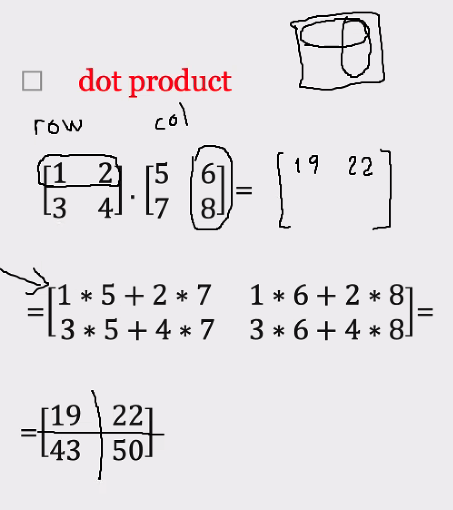
\includegraphics[scale=.5]{fig/1.png}
            \caption{Caption under image}
        \end{center}
    \end{figure}
\newpage
    \subsection{Images side by side}
    \begin{figure}[htb]
        \begin{minipage}[t]{.5\textwidth}
            \centering
            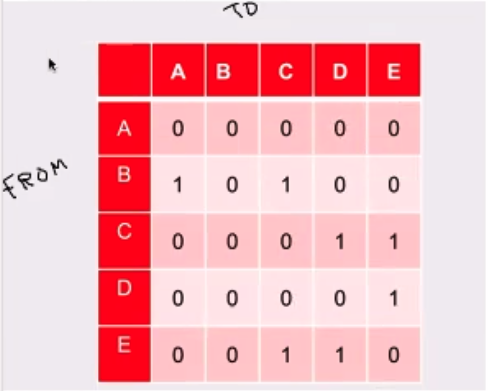
\includegraphics[width=\textwidth]{fig/2.png}
            \caption{Image 1.}\label{fig:2}
        \end{minipage}
        \hfill
        \begin{minipage}[t]{.5\textwidth}
            \centering
            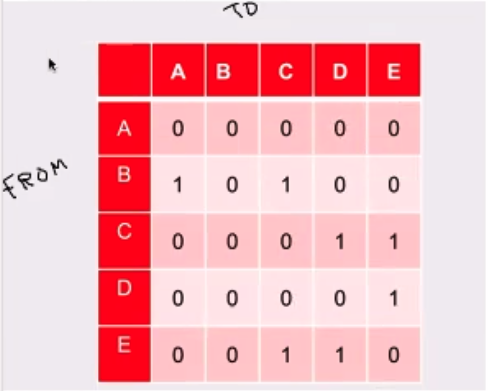
\includegraphics[width=\textwidth]{fig/2.png}
            \caption{Image 2.}\label{fig:3}
        \end{minipage}
        \hfill
    \end{figure}
\newpage
    \section{Referencer til billeder}
    \begin{enumerate}[label=(\alph*)]
        \item Reference til figur \ref{fig:1} på side \pageref{fig:1}
        \item Reference til figur \ref{fig:2} på side \pageref{fig:2}
        \item Reference til figur \ref{fig:3} på side \pageref{fig:3}
    \end{enumerate}
    \section{Section med tal}
    \subsection{SubSection med tal}
    \subsubsection{SubSubSection med tal}
    \subsection{SubSection med tal}
    \section{Section med tal}
    \section{Paragraph}
    \paragraph{Dette er en paragraph}
    \subparagraph{Dette er en sub paragraph}
    \section*{Section uden tal}
    \subsection*{SubSection uden tal}
    \subsubsection*{SubSubSection uden tal}
    \subsection*{SubSection uden tal}
    \section*{Section uden tal}
\newpage
    \section{Lister}
    \subsection{Bullet points}
    \begin{itemize}
        \item Bulletpoint
        \item Bulletpoint
        \item Bulletpoint
    \end{itemize}
    \subsection{Alternative bullet points}
    \begin{itemize}
        \item[--] Bulletpoint
        \item[--] Bulletpoint
        \item[--] Bulletpoint
    \end{itemize}
    \subsection{Enumererede lister}
    \begin{enumerate}[label=(\alph*)]
        \item Bulletpoint
        \item Bulletpoint
        \item Bulletpoint
    \end{enumerate}
\newpage
    \section{Tabeller}
    \begin{table}[hbt!]
        \begin{tabular}{|l|l|l|l|l|}
            \hline
            A1 & B1 & C1 & D1 & E1 \\ \hline
            \multicolumn{3}{|l|}{Left} &  &  \\ \hline
            &  & \multicolumn{3}{r|}{Right} \\ \hline
            \multicolumn{2}{|c|}{Center} &  &  &  \\ \hline
            \multicolumn{2}{|c|}{\multirow{2}{*}{\begin{tabular}[c]{@{}c@{}}Merge\\ Vert\end{tabular}}} & \multirow{2}{*}{} & \multicolumn{2}{c|}{\multirow{2}{*}{\begin{tabular}[c]{@{}c@{}}Merge\\ Vert\end{tabular}}} \\
            \multicolumn{2}{|c|}{} &  & \multicolumn{2}{c|}{} \\ \hline
        \end{tabular}
        \caption{Tabel}\label{tab:1}
    \end{table}
    \section{Reference til tabel}
    Reference til tabel \ref{tab:1} på side \pageref{tab:1}
    \section{Code listing}
    \begin{lstlisting}[language = Java , frame = trBL , firstnumber = last , escapeinside={(*@}{@*)}]
        public class Hello {
            public static void main(String[] args) {
                System.out.println("Hello World");
            }
        }
    \end{lstlisting}
\newpage
    \section{Math}
    \subsection{Inline equations}
    Dette er pythagoras \(a^2 + b^2 = c^2 \) i tekst
    \subsection{Display equations}
    Dette er pythagoras på en \[ a^2 + b^2 = c^2 \]
    seperat linje
    \subsection{Typer}
    \subsubsection{Fractions}
    $\frac{1}{4}$ $\frac{10}{100}$
    \subsubsection{Powers}
    \(x^2 x^3\)
\newpage
    \section{Litteratur}
    \begin{thebibliography}{9}
        \bibitem{latexcompanion} 
        Kate L. Turabian, Wayne C. Booth, Gregory G. Colomb, Joseph M. Williams, Joseph Bizup William, T. FitzGerald. 
        \textit{A Manual for Writers of Research Papers, Theses, and Dissertations}. 
        
        \bibitem{einstein} 
        Elizabeth Tebeaux and Sam Dragga
        [\textit{The Essentials of Technical Communication}]. 
        
        \bibitem{knuthwebsite} 
        \LaTeX,
        \\\texttt{https://tex.stackexchange.com/}
    \end{thebibliography}
\end{document}